\chapter{CUDA Overview}\label{sec:i}
CUDA is a software layer that allow programmers to exploit the capability of nVidia GPUs as general purpose processors.\\
Dealing with a video card in this way requires approaching a completely new programming style and acquiring some knowledge about the basic nVidia GPUs architectures, even though all the internal details are masked by the framework.\\
%First of all, as a philosophical remark, a GPU cannot run anything conceived and written for a CPU, as every vector stream architecture. In order to product software that can be executed on a CUDA Capable GPU, the programmer must write natively parallel code using one of the supported languages, extended with ad hoc CUDA primitives. There is no tool that can perform automatic porting of a sequential code into a parallel one.\\
CUDA exposes the GPU as a "Parallel Co-Processor" that can be used by the CPU to speed-up the computations. More in the details, the CPU - Host - can take advantage of the high amount of parallel threads executable by the GPU - Device - to accelerate parts of a program that are especially well suited for exploiting TLP. According to this approach, the CPU must directly manage the program execution settings on the GPU, provide the data for the computation to the device and collect the outputs when it is done.\\
One of the most important features of CUDA is that it abstracts away all the physical details of the supported GPUs and always shows to the programmer  the very same logical organization (Figure 3.1). These GPUs can be considered a MIMD array of SIMD processors %array of MIMD processors?
, called MultiProcessors. Each MultiProcessor is composed of 3 elements: a fixed number of cores, an instruction unit and a private memory space. All the MultiProcessors share a pubblic memory space referred to as Device Memory in order to distinguish it from the CPU memory space - Host Memory - that is not directly accessed by the GPU. Due to the property of abstraction mentioned before, the only difference between families of nVidia products is in the amount of memory, the number of MultiProcessor and the nature of the cores.\\ %mmh...nn è quello che c'è nell'immagine grigia, però...

\begin{figure}[h!bt]
	\centerline{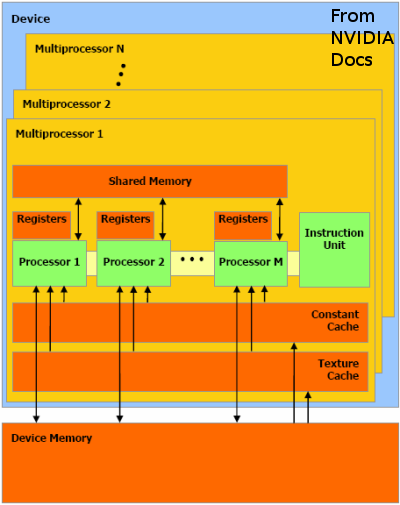
\includegraphics[width=0.5\textwidth]{img/HWModel.png}}
	\caption{Logical Organization of all the CUDA capable devices. The programmer does not have to take care of the physical organization of the GPU that will actually execute the program.}
	\label{fig:nVidiaGPUsLogicalOrg}
\end{figure}

\section{Multiprocessors}
Even if the architectural details of the CUDA capable GPU can significantly differ from a product to another, some common guidelines can be identified.\\
As stated before the MP is a SIMD component: all the SPs belonging to the same MP execute the same instruction on different data. This structure, obviously deigned for graphical purpouses, make the GPUs also particulary effective in addressing problems that can exploit a huge amount of TLP.\\
Form a philosophical point of view, the MPs of these GPUs are designed to be as simple and fast as possible. In order to keep low the complexity, there are neither branch predictors, nor mechanisms to rollback incorrect results. Even if this seems a serious limitation to the performance, it allow the cores of the MP to be completely focused on the arithmetic intensity. As results of this choice, the SPs of the most recent nVidia products are able to perform a double precision MAD (or MUL or ADD) per clock cycle.\\

\section{Memory Hierarchy}
The CUDA memory hierarchy consists of several elements optimized for different memory usages.\\
The Device Memory is the main memory space of the GPU. It can be accessed by both the CPU and the GPU using different policies, usually with a latency of some hundreds of clock cycles. In order improve the performance and the usability, it is logically partitioned into three logic component, depending on the access method: the Global Memory, that follow the common 32-,64-, or 128-byte memory transactions paradigm; Texture Memory, accessed by texture fetching; Constant Memory, managed by special operations.\\
The Global Memory is the most frequently employed memory space. Usually it is used by the CPU to load the data for the computations into the device and by the GPU to provide the results. Furthermore the Global Memory is the only space completely shared among all the SPs of the device: for this reason it is also exploited for comunication among SPs belonging to different MPs. The Texture Memory can be written by the CPU using the CUDA API and readed by the GPU via texture fetching. No GPU texture write mechanism is provided. The Constant memory is a small special memory space that can be used for allocation of variables frequently readed. These variables must be allocated by the CPU before the execution on GPU, that can access them solely in read-only mode.\\ 
Due to the high latency of the Device Memory, each MP is provided with a private low latency memory space, logically divided into:
\begin{itemize}
\item a so called Shared Memory, directly accessible by all the SPs of the MP
\item a Constant Cache and a Texture Cache, managed by the framework
\item a set of exclusive Registers for each SP
\end{itemize}
The Shared Memory can be considered as both a sort of "cache" of the Global Memory %santa potrebbe ucciderci
 directly administrated by the cores in the MP and a mechanism for communicating among SPs belonging to the same MP. The Constant Cache and the Texture Cache are L1 caches used to speed-up the access time of the Constant Memory and the Texture Memory, respectively. Due to the fact that Constant Memory and Texture Memory are read-only (from a GPU point of view), no cache coherency protocol is required.\\ 

\section{Programming Model}
As stated at the beginning of this chapter, the CUDA framework enable the programmer to take advantage of the high number of parallel threads executable by the GPU to expoit TLP: ideally the program is organized into identical sub-problems - working on different data - that can be solved independently. Each of this sub-problems, called Kernels, is mapped onto a thread that will be executed on a SP.\\
All the threads executed by the SPs of a single MP are logically organized into a structure called Block. Virtually speaking, all the Threads belonging to a Block are execuded in parallel. Usually, the number of SPs in a MP is much less than the number of Threads in a Block. For this reason, only a subpart of the Threads is in concurrent execution at a given time - the so called Warp. When a MP is loaded with a Block, it partitions it into warps that get sheduled by a warp sheduler for the execution on that MP. Due to the fact that all the Threads of a Block are executed on the same MP, it should be noticed that they share all the MP resources (i.e. Shared Memory and Caches) and that they can be synchronized using a specific API barriers.\\
All the Blocks are grouped into another logical structure called Grid. Considering that the number of Blocks of the Grid is usually greater than the number of MPs, not all the Blocks can typically be sheduled at the same time. Since the blocks are unordered, they can execute equally well on a GPU that can handle one block at a time and on one that executes a dozen or a hundred at a time, as a demonstration of the scalability offered by the framework. In order to avoid complicating the Block scheduling process, no extra-block threads syncronization mechanism is provided.\\ 

\begin{figure}[h!bt]
	\centerline{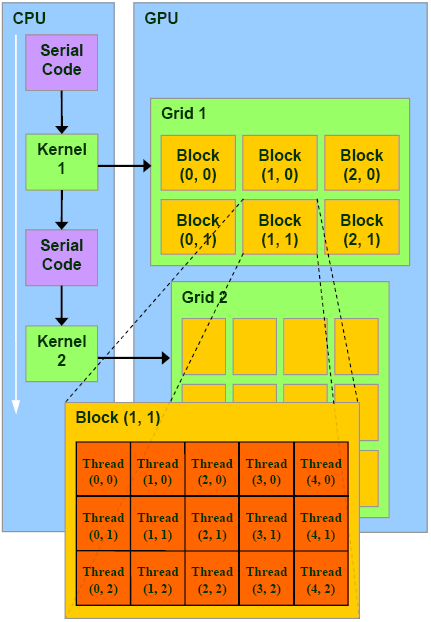
\includegraphics[width=0.5\textwidth]{img/nVidiaExecutionModel.png}}
	\caption{nVidia Execution Model, an example of heterogeneous programming.}
	\label{fig:nVidiaGPUsLogicalOrg}
\end{figure}

\section{Best Pratices}
In order to best exploit the resources of a Cuda capable GPU, there are several pratices that must be adopted. Even if many of these are strictly dependent on the specific device used, there are some general rules that can be easily identified:
\begin{description}
\item[Memory transfers] between Host and Device must be reduced to the minimum. Ideally there should be only one transfer Host-Device to store on the GPU the data for the computation and one transfer Device-Host to collect the results.
\item[GPU Occupancy] must be maximized. That is, the number of warp actually in execution must be closer to the maximum number of "in-fly" warp supported by the Device.\item[Divergent Branches] should be avoided. Due to the fact that all the threads of the warp must execute the same instruction, in case of divergent branches the warp execution will be serialized, reducing the performance.
\end{description}
These three good pratices could be considered the most important rules that must be observed to effective develop in Cuda. It should be noticed that in the past this list was expanded by at least one element, coalescence. In the first Cuda Devices - identified by a so called "compute capability" berween 1.0 and 1.1 - all the threads in the same warp had to access the memory words in sequence and, consequently, to avoiding multiple reads/writes. Only if this pratice was enforced the MP could reduce to the minimum the the number of memory accesses needed to provide the data to all the SPs. With modern devices - compute capability grater or equal to 1.2 - this constraint is much more relaxed: threads can access any worlds in any order, including the same worlds, and a single memory transaction for each segment addressed by the warp is issued. In this cases the problem of coalescence can be completely forgotten.
